% Purpose: Demonstrate relative TikZ layout and distinct implementation styles.
% Status: Draft template; source/status and human layout review pending.
% Source-of-truth: .claude/agents/latex-docxer.md (extracted pipeline diagram).
% Origin: Schematic style samples; solid nodes are not verified project modules.
\documentclass{article}
\usepackage[a4paper,margin=2cm]{geometry}
\usepackage{tikz}
\usetikzlibrary{arrows.meta,positioning,fit,backgrounds,shapes.geometric}
\pgfdeclarelayer{background}
\pgfsetlayers{background,main}
\tikzset{
  base/.style={
    rectangle,rounded corners=3pt,draw=black!80,line width=0.8pt,
    align=center,inner sep=4pt,minimum height=8mm,text width=28mm
  },
  manual/.style={
    base,shape=regular polygon,regular polygon sides=6,
    text width=20mm,fill=orange!10,draw=orange!80!black
  },
  impl/.style={base,fill=blue!8,draw=blue!80!black},
  store/.style={base,fill=gray!10,double,double distance=1pt},
  planned/.style={
    base,fill=gray!4,draw=black!50,
    dash pattern=on 3.5pt off 2.5pt,font=\small\itshape
  },
  arrow/.style={->,thick,draw=black!75},
  plannedarrow/.style={->,thick,dashed,draw=black!50}
}

\begin{document}
\section*{Illustrative pipeline status styles}

\begin{figure}[htbp]
  \centering
  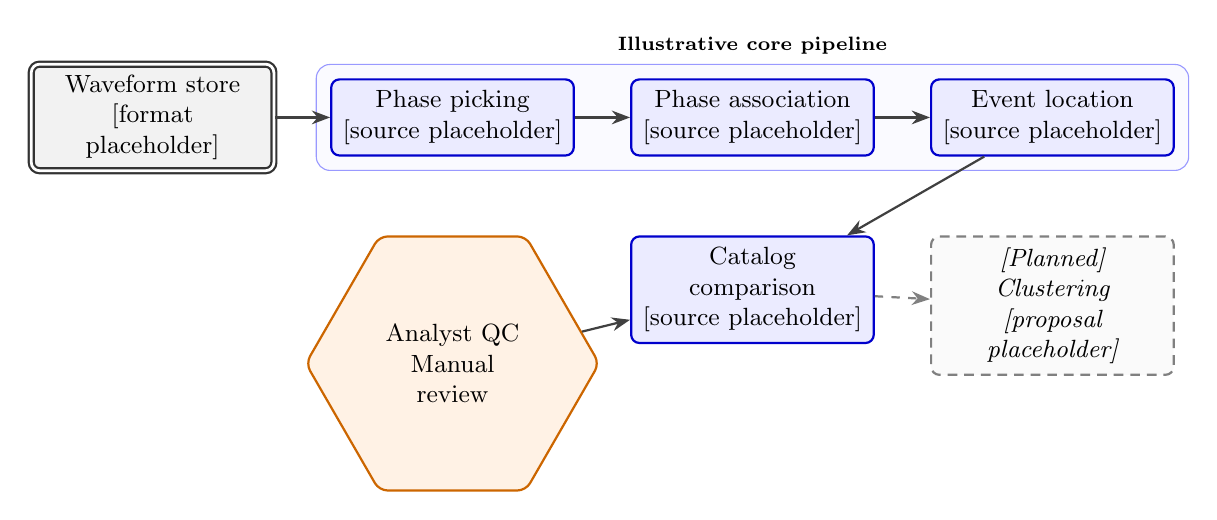
\begin{tikzpicture}[
    >=Stealth,node distance=10mm and 7mm,every node/.style={font=\small}
  ]
    \node[store] (waveforms) {Waveform store\\{[format placeholder]}};
    \node[impl,right=of waveforms] (picking)
      {Phase picking\\{[source placeholder]}};
    \node[impl,right=of picking] (assoc)
      {Phase association\\{[source placeholder]}};
    \node[impl,right=of assoc] (location)
      {Event location\\{[source placeholder]}};
    \node[manual,below=of picking] (analyst) {Analyst QC\\Manual review};
    \node[impl,below=of assoc] (compare)
      {Catalog comparison\\{[source placeholder]}};
    \node[planned,below=of location] (cluster)
      {[Planned] Clustering\\{[proposal placeholder]}};

    \draw[arrow] (waveforms) -- (picking);
    \draw[arrow] (picking) -- (assoc);
    \draw[arrow] (assoc) -- (location);
    \draw[arrow] (analyst) -- (compare);
    \draw[arrow] (location) -- (compare);
    \draw[plannedarrow] (compare) -- (cluster);

    \begin{pgfonlayer}{background}
      \node[
        draw=blue!40,fill=blue!2,rounded corners=5pt,
        fit=(picking) (assoc) (location),inner sep=5pt
      ] (corebox) {};
      \node[anchor=south,font=\scriptsize\bfseries]
        at (corebox.north) {Illustrative core pipeline};
    \end{pgfonlayer}
  \end{tikzpicture}
  \caption{Illustrative seismic-pipeline style key, not an implementation
    claim. Solid blue nodes demonstrate the style reserved for verified
    components; double borders denote storage, the amber hexagon denotes
    analyst review (QC: quality control), and dashed nodes denote planned
    components. Every status is schematic; replace source, storage-format,
    validation, and proposal placeholders using inspected evidence before
    describing a real project.}
  \label{fig:seismology-pipeline}
\end{figure}
\end{document}
